En este capítulo se detallarán las herramientas necesarias para el desarrollo del paquete, como lo son el editor de texto, servidores externos para el entrenamiento del o los modelos, paquetes necesarios para la documentación, distribución, testing y cualquier elemento adicional que sea fundamental para su funcionamiento. A su vez, se especificará la arquitectura del software, haciendo énfasis en los patrones de diseño aplicados y la función de cada módulo o submódulo programado.
\section{Requerimientos mínimos del software}
\begin{itemize}
    \item Las piezas de código debían ser independientes, es decir; si el usuario quisiera aplicar el módulo de reconocimiento debía ser capaz de usar sus funciones sin depender del módulo estéreo y viceversa.
    \item Debía poseer los archivos necesarios para su distribución.
    \item Una sola carpeta que contenga todas las pruebas unitarias del paquete.
    \item Debía ser desarrollado sobre un entorno virtual de python, para poder asegurar que las versiones de los paquetes de los cuales depende, no generen ningún conflicto con las versiones instaladas en el computador de desarrollo, esto en caso de que fuera necesario cambiar el computador de desarrollo en algún punto del proyecto.
    \item No podía ser demasiado pesado por dos razones, la primera se debe a que al ser la versión 1.0 del paquete, implicaría que si en un futuro se publicaran nuevas versiones, el trabajo de optimización de código sería complejo y el segundo motivo es que la herramienta de control de versiones elegida (github) tiene un límite de peso por repositorio de 100 MB, esto restringe el uso de herramientas como ``Tensorflow model API zoo'', ya que sus dependencias elevan demasiado el peso del paquete.
    \item Las funciones del paquete debían poder implementarse de forma simple por cualquier usuario.
\end{itemize}
\section{Entorno de desarrollo}
\subsection{Servidor de Google Colaboratory}
Dado que el computador empleado en la programación del paquete cuenta con una gráfica integrada de recursos insuficientes para el entrenamiento de redes neuronales, se optó por usar los servidores de Google colaboratory o Colab, este no es más que un producto gratuito de Google research que permite a cualquier usuario escribir y ejecutar código de python en el navegador, esta herramienta es un servicio de notebook alojado en Jupyter (aplicación web interactiva para desarrollar software de código abierto) que no requiere configuración previa para usarlo y brinda acceso gratuito a recursos computacionales (GPU y RAM); sin embargo, en el caso de la red entrenada se empleó la versión de pago ``Google colab Pro'' para así tener acceso a una mejor tarjeta gráfica, mayor espacio de almacenamiento, una tarjeta RAM de alta velocidad y eliminar la limitación de tiempo de uso de 12 horas que posee la versión gratuita. Entre las características más importantes de Colab se tiene que:
\begin{itemize}
    \item En Colab los notebooks se almacenan en Google drive, pero también pueden ser cargados desde github, además de poder ser compartidos a cualquier usuario. Aunque esta comunicación no se limita a notebooks, puesto que es posible montar el sistema de archivo de Google drive en un notebook de Colab. Utilizando esta capacidad se guardó el paquete en Google drive y en Colab se procedió a entrenar importando los módulos necesarios, además de que los puntos de guardado y archivos generados en la rutina de entrenamiento se enviaban al almacenamiento de Google drive.
    \item El código es ejecutado en una máquina virtual (VM) exclusiva para la cuenta del usuario, la cuales se borran cuando están inactivas durante un tiempo prolongado o al superar un límite de tiempo de ejecución de 12 horas, este límite de tiempo fue una de las razones por las que se optó por la subscripción paga, ya que; la red requería un mayor tiempo para el entrenamiento.
    \item La cantidad de memoria de la máquina virtual en la versión Pro era de 166.83 GB para el almacenamiento y 25.46 GB de RAM, con estas capacidades fue posible experimentar con el conjunto de datos PASCAL VOC sin problema alguno, puesto que la versión gratuita tendía a alcanzar el límite de memoria con facilidad.
    \item Actualmente cuenta con 4 tipos de GPU que pertenecen a NVIDIA de la serie Tesla la K80, T4, P4 y P100. Aunque no hay una forma de elegir el tipo de GPU a la que se puede conectar el notebook de Colab, todas las opciones disponibles cumplen con las especificaciones suficientes para entrenar modelos de reconocimiento, en el caso de este desarrollo se usó el P100.
\end{itemize}
\subsection{Editor de texto}
Se seleccionó como interfaz de desarrollo, al editor desarrollado y mantenido por Microsoft ``Visual Studio Code'', ya que este posee las siguientes cualidades:
\begin{itemize}
    \item Alternar entre intérpretes de Python, versiones y entornos personalizados, el paquete fue desarrollado en la versión 3.8 de Python.
    \item Ejecutar archivos de python en un terminal de comandos integrado a la interfaz.
    \item La capacidad de configurar y ejecutar pruebas unitarias mediante unos pocos clics.
    \item Es un entorno ligero, ya que los recursos computacionales mínimos son: un procesador de 1.6 GHz, 2 GB de RAM en una arquitectura de 64 bits y 800 MB de espacio disponible en el disco duro.
    \item Una comunidad activa que actualiza y crea nuevas extensiones que mejoran la experiencia del editor.
    \item El soporte continuo de Microsoft y que a pesar de pertenecer a la empresa es una herramienta open source.
    \item La facultad de configurar un Linter que permita detectar el código sospechoso que no cumpla con un formato impuesto o uno personalizado. 
    \item La herramienta IntelliSense cuyas funciones principales son el auto completado y la desambiguación de nombres de variables, funciones y métodos.
\end{itemize}
\section{Estructura del paquete y sus dependencias}
Como se pudo ver en el capítulo II un paquete requiere más que solo el código utilizable para el usuario, si se quiere distribuir en el python package index (PyPI). Por este motivo se estructuró el directorio que contiene al paquete como en la Figura \ref{directorioCompletoPaquete}. 
\begin{figure}[H]
    \centering
    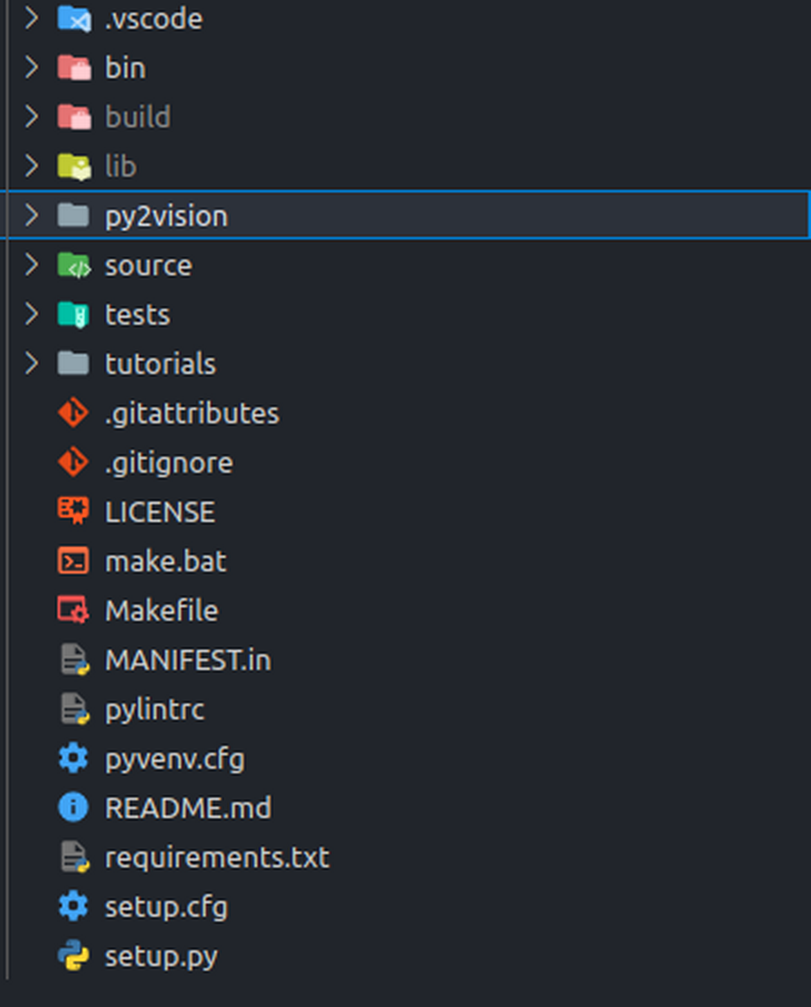
\includegraphics[scale=0.3]{Recursos/directoriosPaqueteNivelRoot.png}
    \caption{Directorio raíz del proyecto}
    \label{directorioCompletoPaquete}
\end{figure}
A continuación se explicará la función de las carpetas y archivos presentes en la Figura \ref{directorioCompletoPaquete}:
\begin{itemize}
    \item \textbf{.vscode:} contiene el archivo json de configuración, generado por el editor de código, el cual le dice al mismo, ciertos ajustes del usuario, tales como: el uso de un Linter, la ubicación del archivo que indica la configuración del Linter, la ubicación o la ruta de la versión de Python, la localización de los test unitarios e incluso el nombre que deben tener los archivos para considerarse test y poder ejecutarlos mediante el editor, en el caso de este paquete son test aquellos archivos cuyo nombre comience por ``test\_''.
    \item \textbf{bin y pyenv.cfg:} bin es una carpeta generada por pyenv, esta es una herramienta empleada para instalar diferentes versiones de Python y cambiar entre ellas según los requerimientos del proyecto en el que se esté trabajando, esto implica que con pyenv es posible crear entornos virtuales que contengan un conjunto de paquetes instalados por el usuario, sin afectar a los paquetes instalados en otros proyectos. Por otro lado, pyenv.cfg es el archivo de configuración que tomara en cuenta la herramienta del mismo nombre al momento de generar la carpeta bin. 
    \\
    \\
    Para activar el entorno virtual es necesario utilizar el siguiente comando en la terminal desde la raíz del proyecto: 
    \begin{verbatim}
        source bin/activate
    \end{verbatim}
    El comando source lee y ejecuta comandos del archivo especificado como argumento en el entorno de shell actual.
    \item \textbf{Makefile, build, source y make.bat:} los dos archivos (Makefile y make.bat) dictan la configuración de la herramienta de documentación ``Sphinx'', la cual puede ser ocupada mediante comandos en la terminal. La carpeta build contiene todas las dependencias configuradas por Sphinx y la carpeta source contiene la estructura de la documentación que puede ser mostrada en distintos formatos, en este caso se eligió un formato html, para que cualquier usuario con un navegador pueda conocer el funcionamiento del paquete.
    \item \textbf{py2vision:} es el nombre del paquete, por lo que esta carpeta contiene los módulos y submódulos de todo el paquete.
    \item \textbf{tests:} contiene los test unitarios aplicados a los módulos y submódulos que se encuentran en la carpeta py2vision.
   \item \textbf{tutorials:} En esta carpeta se encuentran 3 notebooks de Jupyter los cuales pueden ser abiertos con Google Colab y en su interior se encuentran varias lecciones que ejemplifican el uso del paquete. Además alberga un script ejecutable llamado ``stereo\_tuner.py'' que construye una interfaz para ajustar los parámetros del algoritmo de correspondencia empleado en el paquete y un fichero ejecutable llamado get\_anchors\_k\_means.py que permite generar las dimensiones de los anchor boxes utilizados en la detección de objetos analizando la estructura del conjunto de datos mediante el algoritmo de clusterización ``K means''.
    \item \textbf{MANIFEST.in:} cuando se construye el código que será distribuido, Python toma por defecto la carpeta del proyecto; sin embargo, hay algunos archivos que no deben dejarse por fuera, como puede ser el caso del setup.py, README.txt, pyproject.toml y setup.cfg. Para estos casos es que existe el archivo MANIFEST.in, ya que este incluye o excluye los archivos que deben o no deben ser distribuidos.
    \item \textbf{pylintrc:} contiene la configuración del formato que sigue el paquete, en el caso de py2vision se sigue el estilo de Google, el cual puede observarse al detalle en https://google.github.io/styleguide/pyguide.html.
    \item \textbf{setup.cfg:} Como se pudo ver en la Figura \ref{estructuraSetupTools} es un archivo necesario en caso de utilizar Setuptools para la distribución.
    \item \textbf{setup.py:} Es el archivo de configuración en caso de usar Distutils para la distribución, se dejaron ambas opciones de ser necesario uno u otro.
    \item \textbf{requirements.txt:} Es un archivo de texto que contiene los paquetes externos que necesita py2vision para funcionar.
\end{itemize}
\section{Diseño de la arquitectura del paquete}
El paquete ''py2vision'' se encuentra diseñado sobre el lenguaje de programación python y utiliza las siguientes dependencias externas para agilizar y optimizar el desarrollo:
\begin{itemize}
    \item Numpy y pandas: para el manejo algebraico y presentación de los datos.
    \item Opencv-contrib-python: se usa para recibir la entrada de datos y exportar en formatos de vídeo o imagen según sea el caso, así como también para la calibración de las cámaras y realizar el mecanismo estéreo, si el usuario tiene instalada la versión base de este paquete se recomienda desinstalarla e instalar esta, para no ocasionar conflictos de dependencias.
    \item Tensorflow/keras: como framework de machine learning.
    \item wget: se usa cuando es necesario descargar contenido de internet, en esta ocasión se usó para poder descargar archivos que contengan los pesos de una red y así aplicar transferencia de aprendizaje o simplemente recuperar los pesos de la red original empleada.
    \item pyyaml y h5py: ambos son necesarios al entrenar para recuperar los pesos a partir de un punto de guardado.
\end{itemize}
Al adentrarnos en el directorio de py2vision podemos observar la siguiente distribución de carpetas:
\begin{figure}[H]
    \centering
    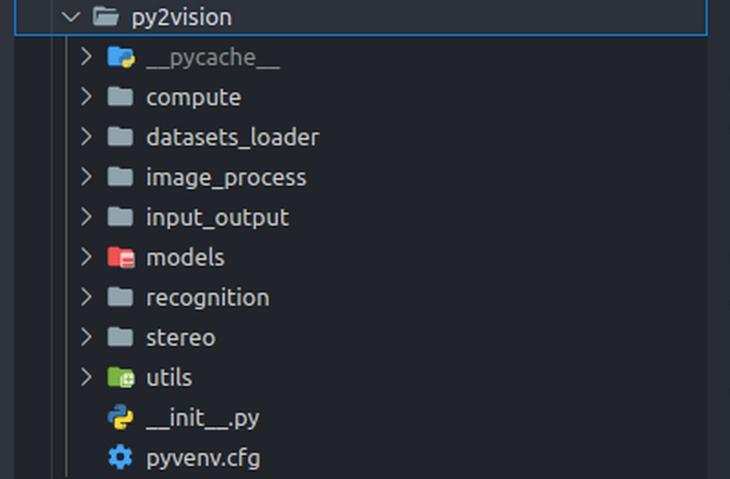
\includegraphics[scale=0.4]{Recursos/pytwovision_folder.jpg}
    \caption{Distribución de la carpeta del proyecto}
    \label{pytwovision_folder}
\end{figure}
Cada carpeta cumple el rol que indica su nombre, sin embargo en breve se explicara a detalle la distribución de clases y métodos, así como también los patrones de diseño y sus funciones.
\subsection{Módulo compute}
Este directorio se creó con el fin de albergar los cálculos que puedan necesitar los mecanismos estéreo y los requeridos por las redes neuronales. Cuenta con los archivos:
\begin{itemize}
    \item \textbf{error\_compute.py}: actualmente cuenta con un solo método llamado \\``re\_projection\_error'', el cual calcula la distancia de la imagen entre un punto proyectado y uno medido. Para lograrlo se calculan las proyecciones 2D de puntos 3D en el plano de imagen, dados los parámetros extrínsecos e intrínsecos de las cámaras, luego se halla el error promedio con la norma L2 como en la ecuación \ref{average_error}.
    \begin{equation}
        \frac{\sqrt{\sum_{I} (img\_point(I) - projected\_point(I))^{2}}}{n} \label{average_error}
    \end{equation}
    donde img\_point(I) son los puntos de referencia, projected\_point(I) son las proyecciones 2D de los puntos 3D y $n$ son la cantidad de puntos proyectados. Puede emplearse para hallar el error de calibración de un sistema estéreo.
    \item \textbf{yolov3\_calculus.py:} contiene la clase ``YoloV3Calculus'' que se encarga de agregar la capa de predicción en una red YOLO versión 3, convertir las matrices que contengan las coordenadas de bounding boxes de un formato ($xmin$, $ymin$, $xmax$, $ymax$) a un formato ($cx$, $cy$, $w$, $h$) donde $cx$ y $cy$ son las coordenadas del punto central del bounding box y las variables $w$ y $h$ son el ancho y el alto del cuadro respectivamente, dicha conversión puede hacerse en ambos sentidos.
    \\
    \\
    También se encarga de calcular el valor del IoU y aplicar el algoritmo de ``Non maximum suppression'' para filtrar los bounding boxes que no cumplan con cierto umbral, con el fin de obtener predicciones con una menor cantidad de ruido y calcular el error de la red.
\end{itemize}
\subsection{Módulo datasets\_loader}
Se elaboró debido a que la forma en que se presentan los conjuntos de datos introducidos en una red puede variar dependiendo del tipo de reconocimiento (sea detección, clasificación o segmentación) e incluso el mecanismo de entrenamiento de cada arquitectura de red varia, en ocasiones requiere un preprocesamiento especial. Por estos motivos en este módulo cada archivo debe contener una clase que adapte el conjunto de datos para poder ser introducido en una red neuronal. Actualmente alberga la clase ``YoloV3DatasetGenerator'', la cual toma las anotaciones de un archivo que contenga las localizaciones de las imágenes del conjunto, sus bounding boxes y la clase a la que pertenece el objeto y las adapta a la red para su entrenamiento y evaluación.  
\subsection{Módulo image\_process}
El concepto de este módulo se basa en poder aplicar diferentes efectos a imágenes de entrada utilizando una clase en común y de ser necesario apilar un efecto sobre otro a dicha imagen. Debido a esto todo el módulo se aprovecha del patrón de diseño de software conocido como ``Decorator'' el cual permite:
\begin{itemize}
    \item Extraer el comportamiento de un objeto sin crear una nueva subclase.
    \item Combinar varios comportamientos envolviendo un objeto con varios decoradores.
    \item Cada clase tiene una sola responsabilidad, lo que hace posible dividir una clase monolítica que implementa muchas variantes posibles de comportamiento, en varias clases más pequeñas, de modo que facilita el agregar un nuevo procesamiento en la imagen.
\end{itemize}
Este directorio se encuentra estructurado de la siguiente manera:
\begin{figure}[H]
    \centering
    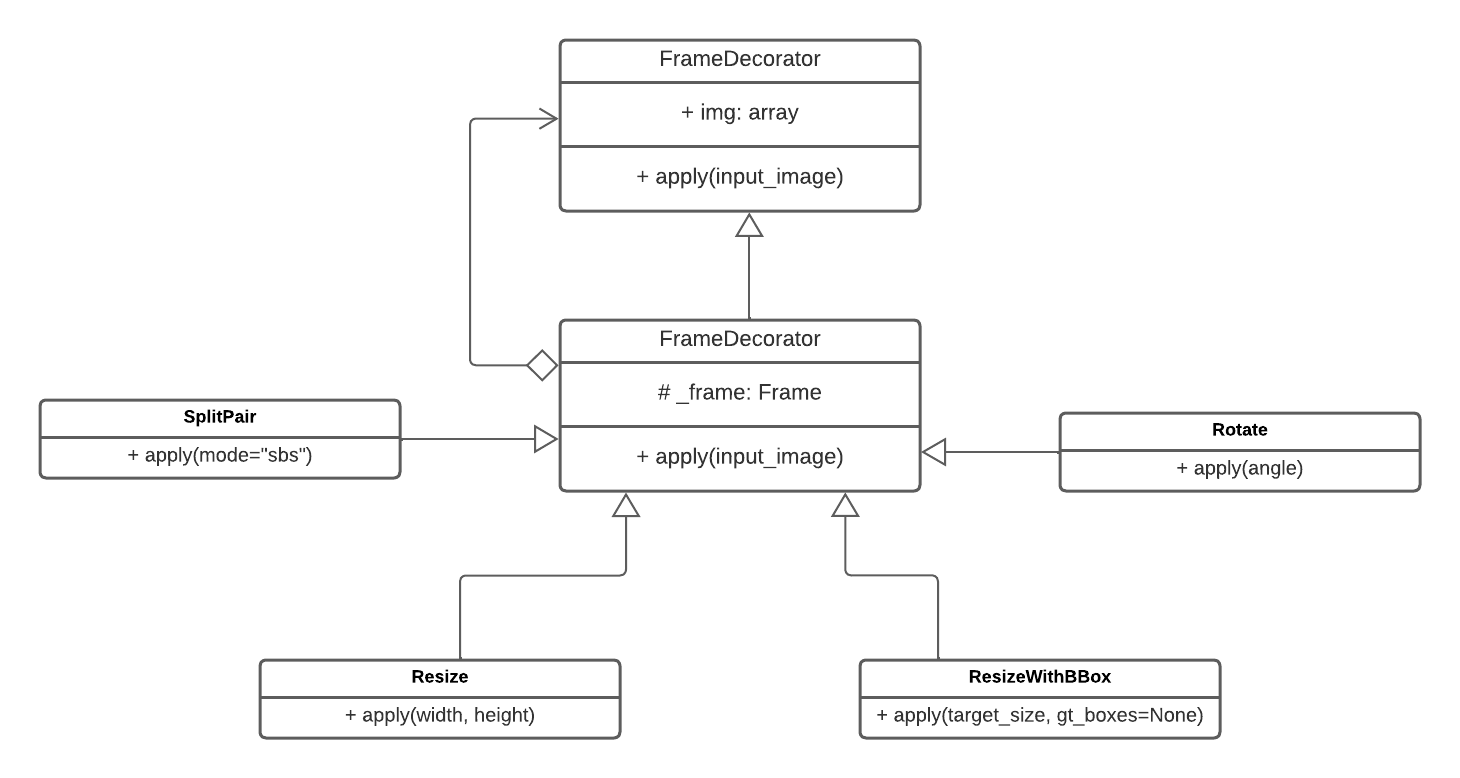
\includegraphics[scale=0.4]{Recursos/image_process_uml.png}
    \caption{Diagrama de clases UML: Módulo image\_process}
    \label{image_process_uml}
\end{figure}
En la Figura \ref{image_process_uml} se puede observar un diagrama que representa las relaciones entre las clases del módulo, los atributos de cada clase ubicados en la sección media de los rectángulos y sus correspondientes métodos (la sección baja de los rectángulos). En este tipo de diagramas se tiene por convención que el símbolo ``+'' indica que un atributo o un método es público, es decir; que desde una clase externa que no herede de la clase anfitriona es posible acceder a dicha variable, mientras que el símbolo ``\#'' indica que es protegida, por lo que subclases que heredan de la clase padre pueden acceder a la variable, pero no es posible acceder a dicha variable desde clases o entornos externos, también existe el símbolo ``-'' implica que la variable es privada por lo que solo es posible acceder a ella desde la clase anfitriona.
\\
\\
En la Figura ya mencionada se puede observar que la clase FrameDecorator hereda de la clase Frame y a su vez tiene una relación de agregación, esto significa que aunque no exista la clase FrameDecorator la clase Frame todavia tiene motivos para existir, ya que podría tener otro decorador base que dependa de ella, el resto de las clases heredan de FrameDecorator y son precisamente los distintos decoradores que aplican los efectos en la imagen de entrada.
\subsection{Módulo utils}
En su interior se encuentran todas aquellas funcionalidades que no encajan en el resto de los módulos, tales como:
\begin{itemize}
    \item \textbf{annotations\_parser.py}: este archivo está basado en el patrón de diseño ``visitor'', debido a que se necesitaba que el sowftware pudiese convertir anotaciones que se encontraran en diferentes formatos (bien sea JSON, XML, txt, etc.) a anotaciones compatibles con los generadores de conjuntos de datos dentro del módulo datasets\_loader. Visitor es un patrón cuya función es separar algoritmos de los objetos sobre los que operan, ofreciendo asi las siguientes ventajas:
    \begin{itemize}
        \item Es posible introducir un nuevo comportamiento que puede funcionar con objetos de clases diferentes sin cambiar esas clases.
        \item Puedes tomar varias versiones del mismo comportamiento y ponerlas en la misma clase.
        \item Un objeto visitante puede acumular cierta información útil mientras trabaja con varios objetos. Esto puede resultar útil cuando quieras atravesar una compleja estructura de objetos, como un árbol de objetos, y aplicar el visitante a cada objeto de esa estructura.
    \end{itemize}
    En la Figura \ref{annotations_parser_uml} se puede apreciar que la interfaz Parser tiene una relación de composición con la interfaz visitante (AnnotationsFormat), lo que implica que Parser necesita de la clase visitante para funcionar. YoloV3AnnotationsFormat implementa el formato de anotaciones compatible con la red del mismo nombre, mientras que XmlParser al heredar de la clase Parser redirige la llamada al método adecuado del visitante correspondiente, en este caso este sería el metodo visit\_xml\_parser(). 
    \begin{figure}[H]
        \centering
        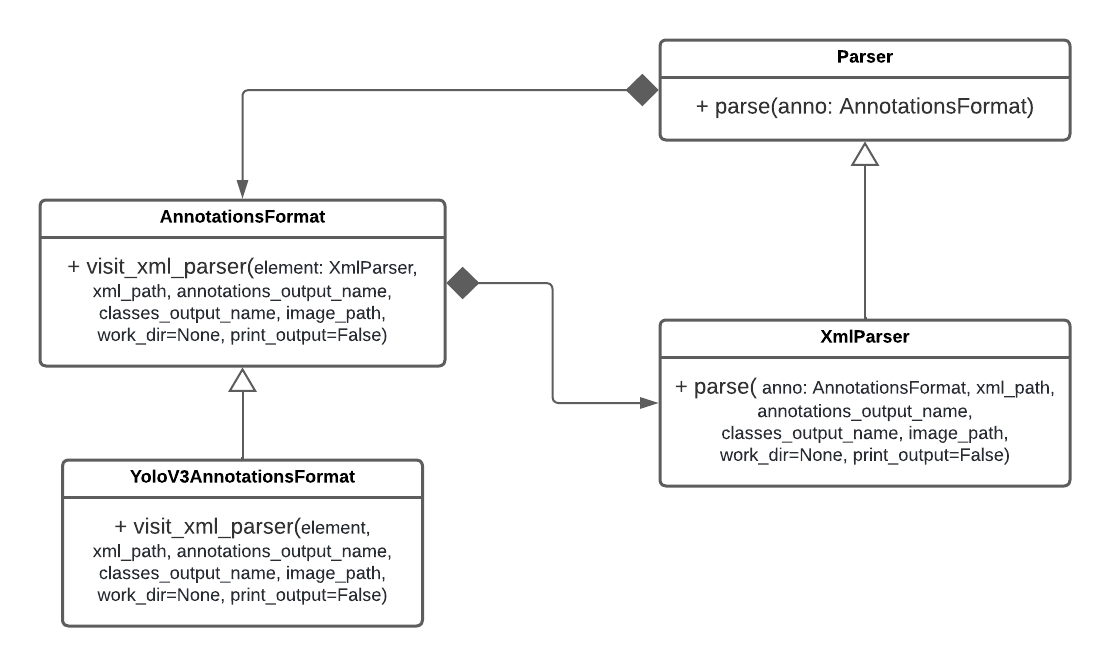
\includegraphics[scale=0.5]{Recursos/annotations_parser_uml.png}
        \caption{Diagrama de clases UML: annotations\_parser}
        \label{annotations_parser_uml}
    \end{figure}
    \item \textbf{annotations\_helper.py:} contiene una clase llamada AnnotationsHelper, la cual recibe como entrada la localización de las anotaciones generadas por annotations\_parser.py y las convierte en variables del tipo Dataframe las cuales pueden ser manipuladas por la librería pandas, para luego separar el conjunto de datos en dos partes e incluso generar los archivos de anotaciones de cada una.
    \item \textbf{draw.py:} posee un método que dibuja las líneas epipolares captadas a partir de dos imágenes y otro que traza los bounding boxes en una imagen.
    \item \textbf{gen\_pattern.py:} crea un archivo svg con el patrón de calibración estéreo, ya sea; un patrón de cuadros de ajedrez o un patrón en forma de círculos.
    \item \textbf{label\_utils.py:} alberga métodos que contribuyen con el funcionamiento de los generadores de conjuntos de datos en datasets\_loader.
\end{itemize}
\subsection{Módulo models}
Se ocupa de generar las capas y bloques que conforman las arquitecturas de las diferentes redes neuronales utilizando las herramientas que ofrece Tensorflow. Dentro de models hay dos submódulos blocks y layers, el primero almacena agrupaciones de capas, las cuales pueden ser propias de Tensorflow o capas personalizadas las cuales se encuentran en el submódulo layers. 
\\
\\
En este módulo hay dos patrones de diseño el primero está en el submódulo blocks en el archivo backbone\_block.py, este emplea el patrón ``Strategy'' para separar los algoritmos de arquitecturas de red conocidas como backbones networks, las cuales son redes que fungen como extractores de características (features) sobre sus datos de entrada. Este patrón da las siguientes ventajas:
\begin{itemize}
    \item Aislá los detalles de implementación de un algoritmo del código que lo utiliza.
    \item Sustituye la herencia por composición.
    \item Se pueden introducir nuevas estrategias sin tener que cambiar el contexto, que en este caso es la clase BackboneBlock de la Figura \ref{backbone_block_uml}.
\end{itemize}
\begin{figure}[H]
    \centering
    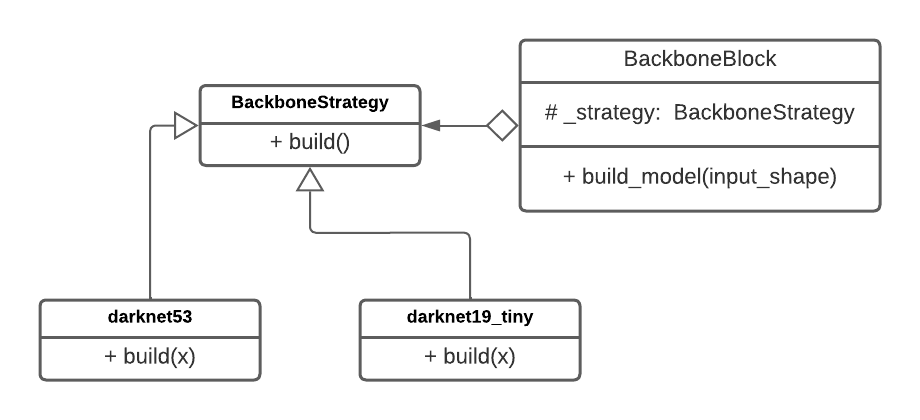
\includegraphics[scale=0.5]{Recursos/backbone_block_uml.png}
    \caption{Diagrama de clases UML: backbone\_block}
    \label{backbone_block_uml}
\end{figure}
Como se puede ver en la Figura \ref{backbone_block_uml} hay dos estrategias que heredan del contexto, sin embargo de ser necesario es posible implementar más con solo agregar la clase de la estrategia correspondiente.
\\
\\ 
Dado que la cantidad de arquitecturas de red existentes para realizar reconocimiento es enorme, se requería una forma de organizarlas sin generar dependencias caóticas entre objetos, por este motivo se empleó el segundo patrón de este módulo, el cual es conocido como ``Mediator'' este restringe las comunicaciones directas entre objetos forzándolos a colaborar únicamente a través de un objeto mediador, el cual como se puede ver en la Figura \ref{models_manager_uml} se representa con la interfaz ModelManagerInterface y su mediador concreto es ModelManager, ya que este almacena todos los modelos de red programados en el software.
\begin{figure}[H]
    \centering
    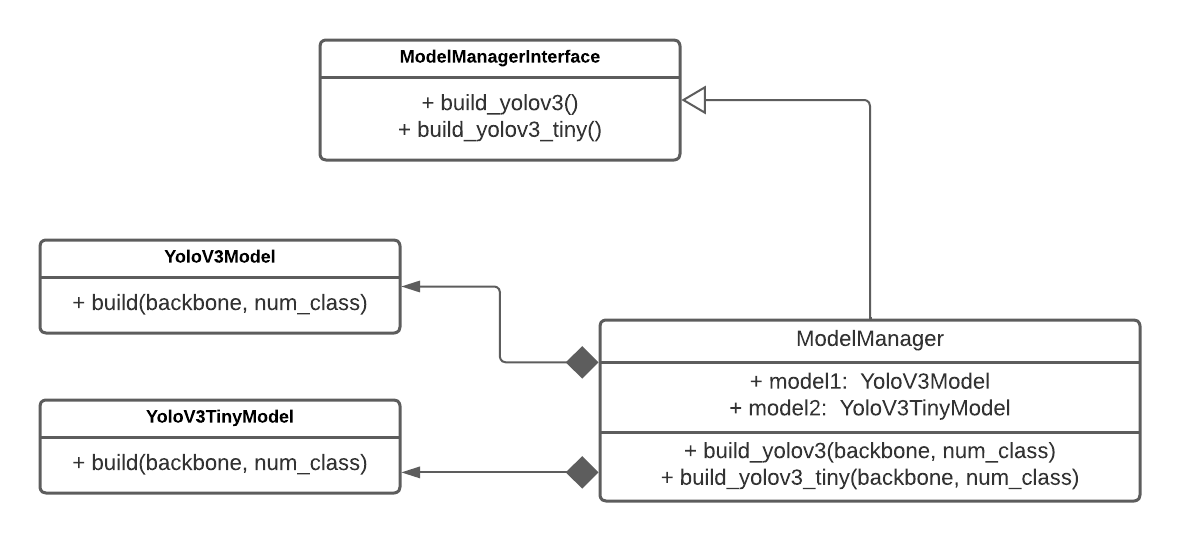
\includegraphics[scale=0.5]{Recursos/Model_Manager_uml.png}
    \caption{Diagrama de clases UML: models\_manager}
    \label{models_manager_uml}
\end{figure}
\subsection{Módulo recognition}
Utiliza el patrón ``Bridge'' para separar la abstracción usada por el usuario, del flujo de trabajo de una red neuronal que engloba el entrenamiento, inferencia, imprimir la estructura de la red, evaluarla y recuperar los pesos pre-entrenados (ver Figura \ref{bridge_uml}).
\begin{figure}[H]
     \centering
     \begin{subfigure}[b]{0.4\textwidth}
        \centering
        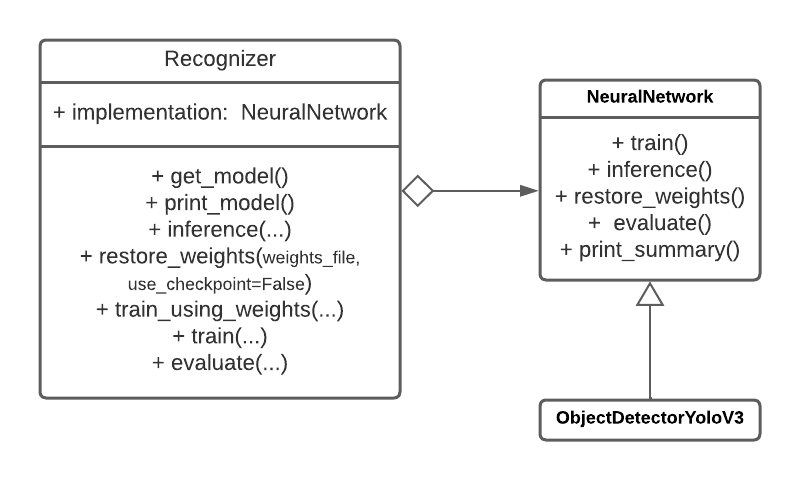
\includegraphics[scale=0.4]{Recursos/bridge_uml.png}
        \caption{Patrón bridge en archivo selector}
        \label{bridge_uml}
     \end{subfigure}
     \hspace{1em}
     \begin{subfigure}[b]{0.4\textwidth}
         \centering
        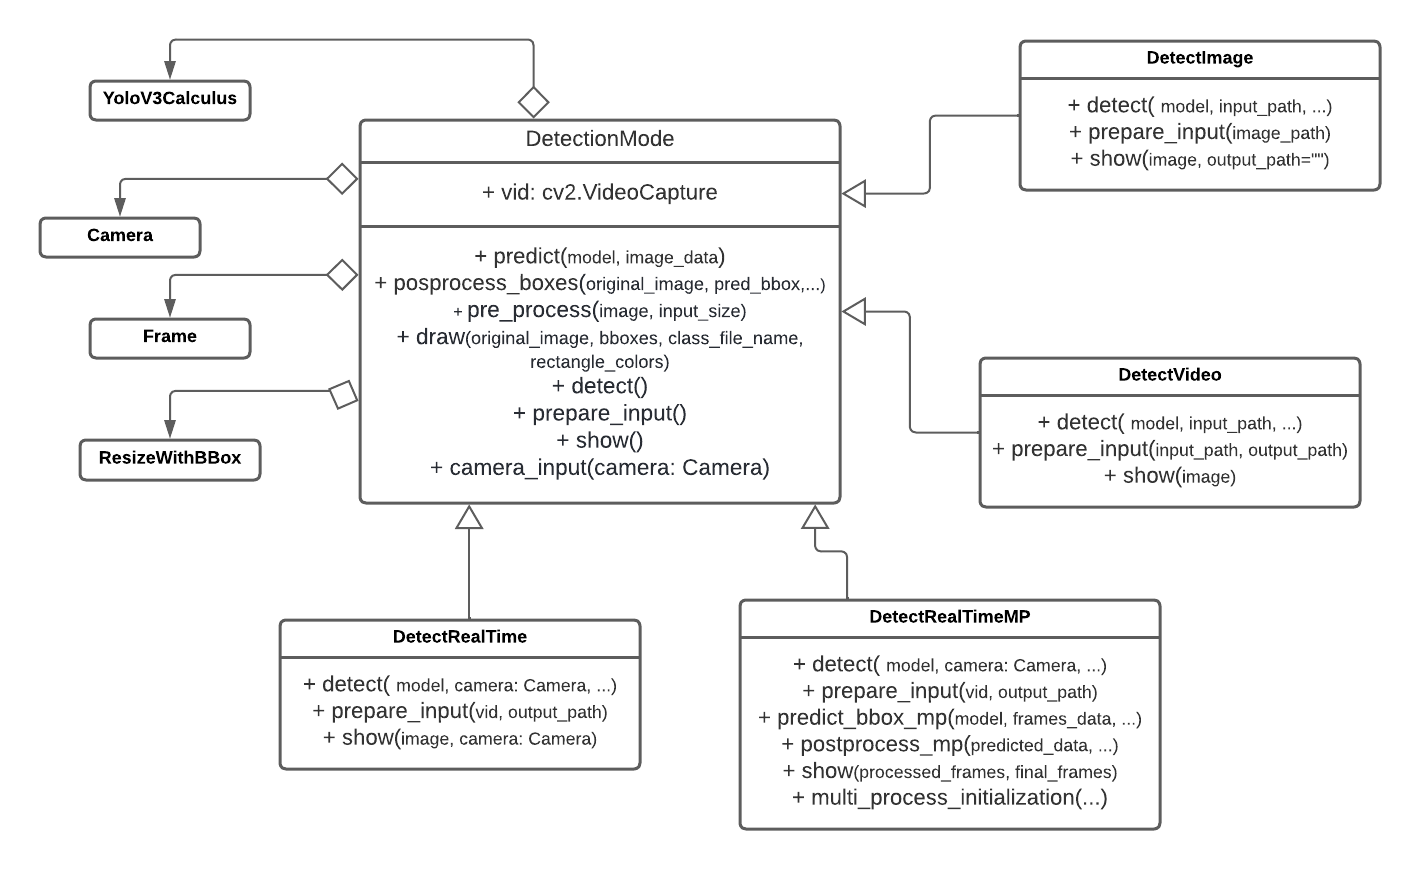
\includegraphics[scale=0.4]{Recursos/template_method_uml.png}
        \caption{Patrón template method en archivo detection\_mode}
        \label{template_method_uml}
     \end{subfigure}
     \hspace{1em}
\caption{Diagramas de clases UML: Módulo recognition}
\label{recognition_umls}
\end{figure}
También en el archivo detection\_mode se aplicó el patrón ``Template method'' de la Figura \ref{template_method_uml}, dado que; este fichero contiene 4 formas de inferencia: a tiempo real, utilizando multiprocesamiento, cuando la entrada es un archivo mp4 y cuando la entrada es una imagen. Sin embargo estas 4 formas comparten algunos procesos en común y su estructura es similar, por esto para poder maximizar la reutilización de código se eligió dicho patrón, a la vez que permite separar en métodos cada etapa de la inferencia.
\subsection{Módulo stereo}
Este comprende el mecanismo estéreo del cual se hablara en el siguiente capítulo. El primer patrón que ocupa es ``Strategy'' para elegir la metodología de correspondencia, en la Figura \ref{strategy_matcher_uml} se puede observar que actualmente existe solo una estrategia (StereoSGBM), sin embargo el patrón es capaz de aceptar ``n'' metodologías de correspondencia. 
\begin{figure}[H]
    \centering
    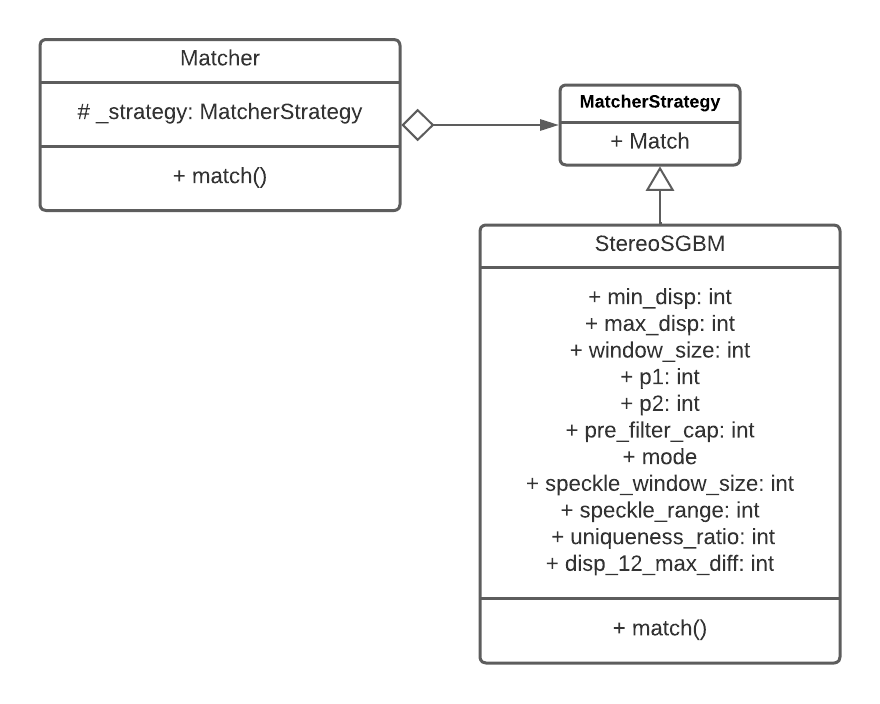
\includegraphics[scale=0.5]{Recursos/strategy_matcher_uml.png}
    \caption{Diagramas de clases UML: en fichero match\_method}
    \label{strategy_matcher_uml}
\end{figure}
El segundo patrón es ``Builder'' el cual se implementa en la Figura \ref{builder_stereo_uml}, en esta se aprecia que StereoController es la clase directora, la cual define el orden en el que se invocarán los pasos de construcción, por lo que puedes crear y reutilizar configuraciones específicas de los productos (StandardStereo). La interfaz constructora (StereoSystemBuilder) declara los pasos de construcción del producto que todos los tipos de objetos constructores tienen en común. El constructor concreto (StandardStereoBuilder) ofrece una implementación del mecanismo estereo.
\begin{figure}[H]
    \centering
    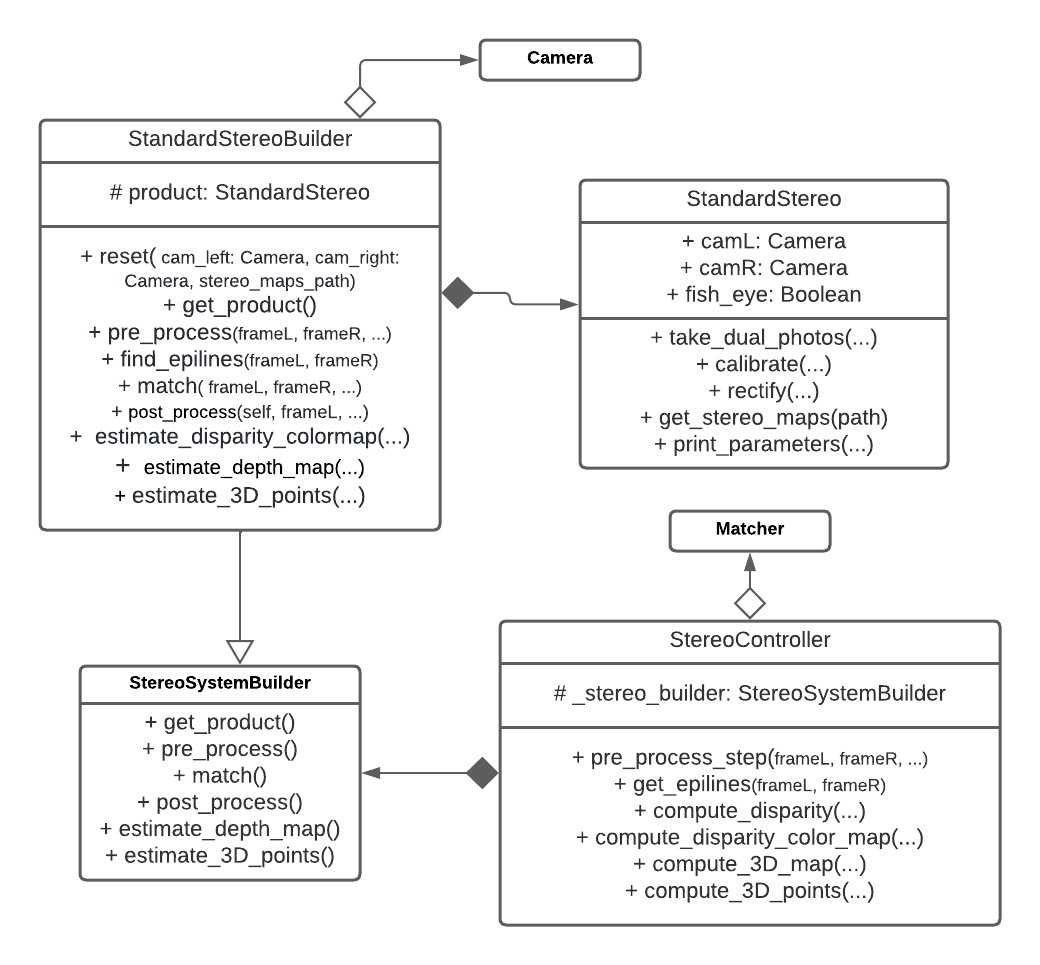
\includegraphics[scale=0.5]{Recursos/builder_uml.png}
    \caption{Diagrama de clases UML: mecanismo estéreo}
    \label{builder_stereo_uml}
\end{figure}
\subsection{Módulo input\_output}
Se diseñó con el fin de contener las clases que permiten la entrada de datos al sistema estéreo y de reconocimiento a través de hardware externo bien sean cámaras, archivos de video o incluso transmisión en vivo mediante wifi, además de obtener los parámetros intrínsecos e extrínsecos del medio físico que capturo las imágenes. Por otro lado, su otra función es fusionar las capacidades del módulo recognition y el módulo stereo en el archivo vision\_system.py que alberga la clase del mismo nombre, la cual ejecuta el algoritmo de posicionamiento cuando la entrada es video o imágenes, de tal forma que se obtenga la salida correspondiente.